\chapter{Implementation\label{cha:chapter4}}
The previous chapters have established the foundation for this thesis. The need for anonymization granularity in distributed event stores has been discussed in chapter \ref{cha:chapter1}. The existing literature and research were provided in chapter \ref{cha:chapter2} with an emphasis on anonymization techniques specifically for streaming data. Chapter \ref{cha:chapter3} served as an outline of the expected functionality of the system. This chapter focuses on the practical steps taken to materialize the aforementioned system, detailing the technological choices, development processes, and the resulting product.\par

This chapter begins with an explanation of the choice of Apache Kafka as a Distributed Event Store, Kafka's architecture, and where the implementation ties in. The subsequent section will focus on the administration of Apache Kafka. This administration is managed through the Apache ZooKeeper framework. Abstracting from the existing \acp{ACL} to enable Role Based Access Control is achieved by the \ac{RBAC} system. How this is done will be the center of the next section. Next, the focus shifts to the central component of the implementation: the Anonymization Stream Factory. We will go in-depth on its various components, illuminate the thought process, highlight its core features, and explain how it can be adapted going forward. For effective testing of the system, a data pipeline has been constructed using the aforementioned components. To complete the pipeline we have added a Data Generator, a Kafka Connector, and a Kafka Consumer. They will be the focal point of the Test Suite section. Finally, the concluding section will demonstrate the integration of these components into a cohesive system, facilitated by Docker for ease of use and deployment.

\section{Distributed Event Store - Apache Kafka}
Out of the multitude of distributed event stores available, Apache Kafka has been selected for this research. Its scalability and reliability, while maintaining low latency and high throughput have established Kafka as the de facto standard in message broking. Combined with its compatibility with essentially all stream processing frameworks, albeit offering its stream processing framework Kafka Streams, Kafka is one of the leaders in big data processing technologies worldwide. Its utilization spans multiple sectors, including Fortune 100 companies, governments, and healthcare. Furthermore, as an open-source technology, Apache Kafka offers a rich set of tools and an active community. This allows a more thorough exploration of practical implementations simultaneously staying grounded in real-world applicability. Although there are noteworthy competitors such as Apache Hadoop, Amazon Kinesis, or RabbitMQ, ultimately Kafka aligns best with the requirements at hand, particularly due to its extensive support for research and development endeavors.

\subsection{Architecture}
So let us take a look at Kafka's architecture shown in Figure \ref{fig:kafka}. There is quite a bit of Kafka terminology involved, in the following written in cursive. 

\begin{figure}[ht]
   \begin{adjustbox}{center}
   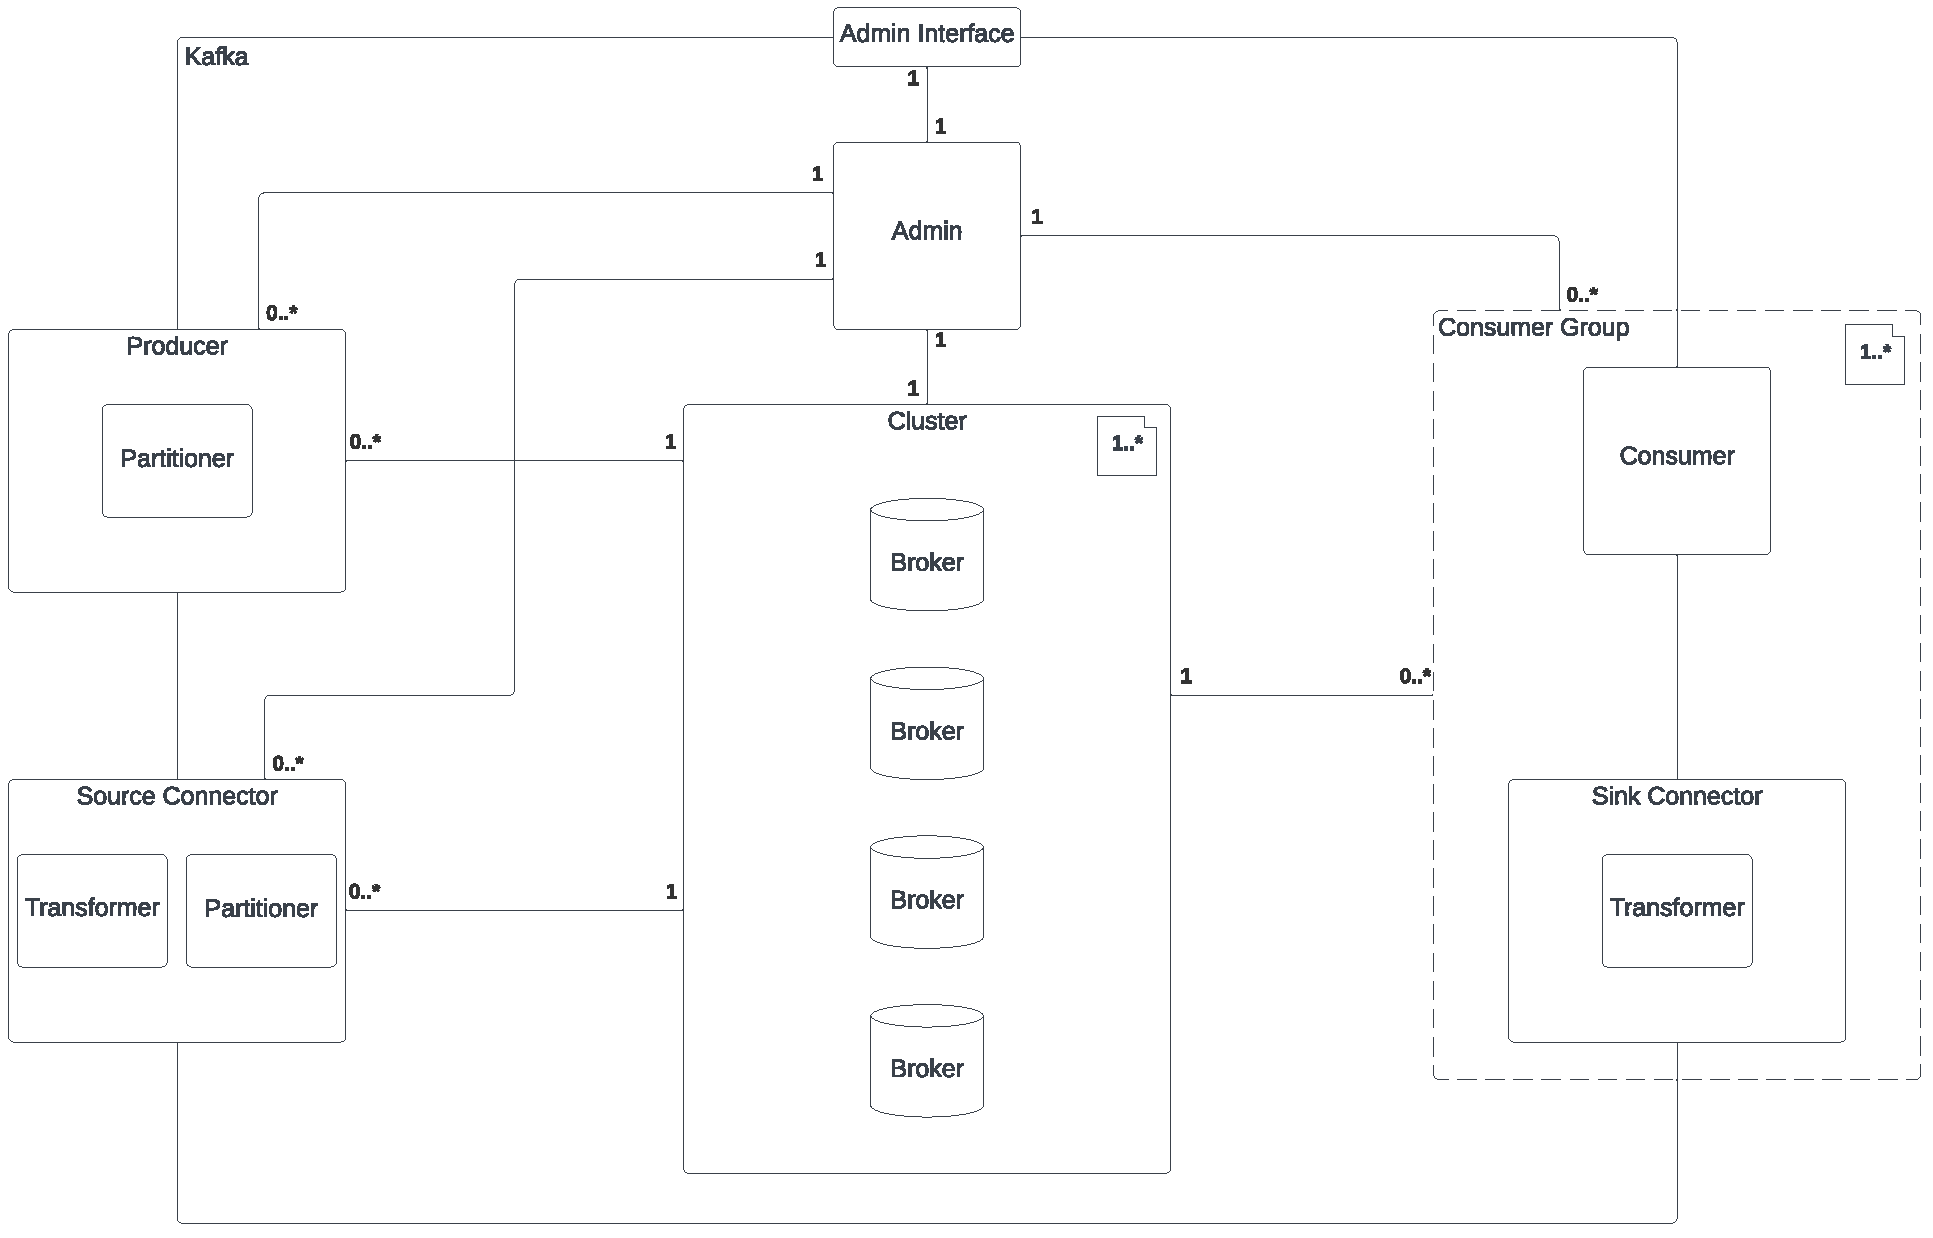
\includegraphics[width=0.8\pdfpagewidth]{img/Kafka_Diagram.pdf}
   \end{adjustbox}
   \caption{Apache Kafka Architecture and Terminology. The links between components have been enhanced with cardinalities to provide more context. \label{fig:kafka}}
\end{figure}

At the core is the \textit{Cluster}, containing at least one \textit{Broker} (database), this is denoted with the note in the top right corner reading '1..*'. As a cluster, they function as distributed storage. However, they deal exclusively with streaming data. A singular stream of related events is termed \textit{Topic}, produced and distributed across the individual Brokers according to strategies delineated by the administration component. For topic production, a \textit{Producer} must be developed by the user to format the raw data. Alternatively, users can employ \textit{Connectors} that interface external systems with Kafka, thus relieving users of data transformation tasks. These connectors are available in a plug-and-play fashion, and the \textit{Kafka Connect} framework allows for the creation of custom connectors. \textit{Consumers} retrieve topics, operating collectively within \textit{Consumer Groups}. Kafka provides three distinct delivery semantics — 'at least once', 'at most once', and 'exactly once' — which refer to how often a singular event is delivered to each consumer group. On the consumer side, similarly to Producers, a \textit{Kafka Consumer} requires user development, although connectors for integrating Kafka with external systems are available. Note that custom Consumers and Connectors can coexist in on Consumer Group. The administration is available through a \textit{Kafka Admin} framework. However, simply using the Kafka Admin framework requires significant development overhead. Instead, other frameworks are brought in to adopt this task. 

\subsection{Administration}
There are several tasks that the administration unit of Kafka has to accomplish. These administrative tasks must be made configurable for the system administrator within the Kafka environment. The responsibilities include the following: 

\begin{enumerate}
   \item \textbf{Cluster configuration}\\It must be in close communication with the brokers. It must be possible to add and delete individual brokers to the cluster.
   \item \textbf{Topic Control}\\Topics must be creatable and deletable. Topics are associated with producers and consumer groups. In particular, the offsets for consumer groups must be monitored. Typically, this is done in an additional "consumer offsets" topic. Here consumer groups are mapped to their offset. Consumer groups periodically publish on this specific topic whenever they consume messages from their respective topics.  
   \item \textbf{Partition Strategy}\\The partition strategy for producers must be communicated. Partitions need to be assigned to brokers. 
   \item \textbf{Replication Strategy}\\To ensure reliability partitions need to be replicated. There is a partition leader stored on one broker and replications on several other brokers. The administration must be able to select the replication strategy.
   \item \textbf{Access Control}\\Access control must be enforceable for producers, consumers, and particularly for administrative operations.  
   \item \textbf{Fault-tolerant}\\The administration component itself must be robust and reliable.
\end{enumerate}

While technically all these requirements can be met simply using the Kafka Admin framework, Kafka themselves do not recommend it. Up until Kafka Version 3.3 (released in August 2022), Kafka advised the delegation of the administration to another framework called \textit{Apache ZooKeeper}. ZooKeeper is an open-source centralized service for synchronizing distributed systems, maintaining configuration information, and providing group services. It facilitates the communication of the various components with each other through hierarchical namespaces. Each namespace corresponds to a node within a hierarchical tree structure. A node on its own can simultaneously have children and data. As ZooKeeper is designed for configuration information the data associated with a node is expected to be small (Byte to Kilobyte in size). For instance, ZooKeeper creates nodes for each broker and stores its configuration as data. In a separate node, it stores information about each topic including its partitions, the assignments of partitions to brokers, and the replication logic. These correlations enable ZooKeeper to maintain system operations and adapt to changes. Each node also encompasses a \ac{ACL} that governs the access to the node's data and its children. The change of the ACL of a topic node for instance would affect the access control for the consumption of that topic. ZooKeeper relies on replication to ensure fault tolerance. In addition, watches are created to detect failures in individual nodes. With all this in place, ZooKeeper makes the following guarantees: Sequential Consistency, Atomicity, Single System Image, Reliability and Timeliness. Altogether, it provides all responsibilities as described in the prior.\par
Apache Kafka, however, has created its own administration component called \textit{KRaft}. Instead of administering the cluster externally, it delegates this responsibility to the brokers. They store the necessary metadata for maintenance and administration alongside the topic partitions. Again replication and partition are utilized to ensure durability. This approach significantly reduces overhead, as it obviates the need to maintain and store separate ZooKeeper nodes. KRaft has been introduced in Kafka Version 3.3 and is production ready as of Version 3.5 (released June 2023). However, it may be reasonably anticipated that the adoption of this new administrative approach within production servers will occur over several years.

\subsection{Configuration}
In the Implementation, we use the current newest stable version of Kafka 3.5.1. We opt to use ZooKeeper as Administration as in current production environments it is the standard. For the test suite, a data generator is created, and a custom Kafka Connector is developed to produce data for the cluster. Additionally, a Kafka Consumer is instantiated to validate the anonymized output. The implementation employs the Admin, Connect, and Streams APIs, all of which are version 3.5.1. Further details on the implementation will be provided in the appropriate sections. 


\section{Role Based Access Control}


\section{DASH - Data Anonymization Stream Handler}
Integral to the system is the anonymization of the data stream. This led to the conceptualization of the Anonymization Stream Factory, as introduced in Section \ref{sec:model_architecture}. Its main tasks are threefold: First, it must understand the anonymization granularity relayed in the requirements input by the user. Second, it must apply these requirements to separate anonymized streams. Third, it must provide an interface to monitor and manipulate the streams. Additionally, the success of this component is critically dependent on its reliability, adaptability, and performance. To fulfill these tasks, the \acf{DASH} was developed. The following subsection will provide a comprehensive analysis of \ac{DASH}, addressing its functionalities, interactions, and thought processes that went into its development. \ac{DASH} was developed with Java (Version 11), selected due to Kafka's implementation in Java, thus offering more comprehensive and up-to-date support. A UML Class Diagram was created and will assist in explaining the implementation. It can be found in full in Figure \ref{fig:full_class_diagram} in Appendix A. However, as it spans multiple pages, we will only include excerpts of it in the subsections. 

\subsection{Overview of Anonymization Techniques}
In chapter \ref{cha:chapter2} we have detailed various anonymization techniques. In the subsequent chapter \ref{cha:chapter3} we have categorized them into more comprehensible groups. Based on that we have implemented the vast majority of anonymization techniques and made them available in \ac{DASH}. They are elaborated in Table \ref{table:anonymizer_parameters}. The anonymization techniques are color-coded to show their corresponding anonymization category. Each anonymizer needs some parameters specified for configuration, these are detailed in the table as well. This includes their format or type, whether they are required for the configuration or optional, and a short description of the parameter. Among the value-based anonymization techniques, highlighted in blue, we implemented all but one in \ac{DASH}, Tokenization. Tokenization requires a database as an input parameter and the development overhead for the creation, validation, and testing of such a database was not in the scope of this thesis.\par 
The green highlighted tuple-based anonymization technique conditional substitution is included in \ac{DASH}. This technique supports three distinct kinds of conditions: value matches, numerical ranges, and regular expressions, thereby enhancing its versatility in application.\par 
The red highlighted implemented attribute-based anonymization techniques include Aggregation, its specialization Univariate Microaggregation, and Shuffling. As attribute-based anonymization techniques, they operate on a collection of tuples. \ac{DASH} creates discrete sets of tuples by cutting up the data stream, a technique called windowing. Kafka supports this inherently. There are different kinds of windows available. \ac{DASH} can be configured to work with different kinds of windowing techniques per anonymization stream. The available window types are tumbling and sliding. Both are fixed size, as specified by the required windowSize parameter. Sliding in comparison to tumbling allows the overlapping of windows. A tuple in a sliding window can therefore be included in more than one window, whereas in a tumbling window, it can only be included in one. By setting only the windowSize parameter, the user specifies the window size of a tumbling window. The specification of the optional advance time turns that into a sliding window that moves along the time axis according to that parameter, creating new windows for every advance time unit. Additionally, a grace period can optionally be set. As data streams operate in real-time tuples can be delayed in their transition to the system. A late-arriving tuple can be identified by its associated timestamp and stream position. If the grace period is specified a window waits that amount of time before forwarding the tuples to processing to allow for latecomers to be included. Grace periods are available for both tumbling and sliding windows. These window configurations apply to all attribute-based anonymization techniques. Aggregation and Univariate Microaggregation operate on numerical attributes and aggregate the attributes specified in the 'keys' parameters within a window. Aggregation offers various modes: sum, median, average max, min, count, and mode. It replaces the values of these attributes with the computed values of the specified modes (count refers to the number of tuples within the window; mode refers to the most frequent value within the window). The Univariate Microaggregation is implemented as detailed in Algorithm \ref{algo:uniMicroAgg}. Shuffling can be additionally configured with a seed, making it deterministic. In the case that there are multiple keys to shuffle it can both shuffle them together, ensuring that the content of these attributes remain together after the shuffle, or independently. \par
Finally, the table-based anonymization technique is highlighted in yellow. It includes the implementation of CASTLE's k-anonymization as specified in \ref{lit:castle}. Here, the tuples are processed one at a time instead of windowed as in the attribute-based anonymization techniques. Even though they are entering \ac{DASH} one at a time, they are grouped in static clusters and are only released after expiration as determined by the delta parameter in CASTLE. The implementation requires the Data Officer to specify multiple parameters. Most are simply positive integers defining different aspects of the algorithm. Additionally, the attributes containing \ac{PII} are included to be suppressed. Finally, the quasi-identifiers have to be specified. Remember, these are the attributes that the k-anonymization is applied to. Any set of k entries in the output stream must be indistinguishable concerning their quasi-identifiers. These are generalized and not suppressed to minimize information loss. The 'quasiIdentifiers' parameter is a List containing a String and GeneralizationHierarchy for each quasi-identifier. The String is the attribute name. The 'GeneralizationHierarchy' is a special data structure designed for the implementation of CASTLE. It can take on two forms for the two types of attributes - numerical and categorical. A numerical generalization is specified through a numerical range as well as the bucket size and in its generalization logic equals bucketizing. The categorical attribute requires a generalization tree. Each node has two attributes - the value, e.g. the generalization of that node, and its children, e.g. an array of nodes. \ac{DASH} then applies the algorithms described in CASTLE. The extension to l-diversity was not implemented in \ac{DASH}, but it already provides the bulk of the code necessary including various data structures and methods. However, it was not within the scope of this thesis. Similarly, further extensions to facilitate t-closeness were also excluded from the scope of this thesis. It was decided against implementing Multivariate Microaggregation as there is no optimal algorithm available at this time. 

\pagebreak
\setlength{\LTleft}{-40pt}    
\setlength{\LTright}{-20pt} 
\footnotesize{
   \renewcommand{\arraystretch}{1.5}
      \begin{longtable}{|C{2.5cm}|C{2.5cm}|C{2.5cm}|C{2.5cm}|C{1.6cm}|L{3.5cm}|}
         \caption{
            List of Anonymizers available in the \acf{DASH}. 
            They are listed with their respective category color coded as well as their parameters including the parameter type and whether it is required or not. 
            A description of the parameters is also added.\label{table:anonymizer_parameters}
         } \\
         \hline
         \textbf{Category} & \textbf{Anonymizer} & \textbf{Parameter} & \textbf{Type} & \textbf{Required} & \multicolumn{1}{c|}{\textbf{Description}} \\
         \hline
         \endfirsthead
         \multicolumn{6}{c}%
         {\tablename\ \thetable\ -- \textit{Continued from previous page}} \\
         \hline
         \textbf{Category} & \textbf{Anonymizer} & \textbf{Parameters} & \textbf{Type} & \textbf{Required} & \multicolumn{1}{c|}{\textbf{Description}} \\
         \hline
         \endhead
         \hline \multicolumn{6}{r}{\textit{Continued on next page}} \\
         \endfoot
         \hline
         \endlastfoot

         \cellcolor{lightblue} ValueBased & Blurring & keys & List\textless String\textgreater & \checkmark & List of attribute names to blur\\
         \cline{3-6}
         \cellcolor{lightblue} & & nFields & positive integer & $\times$ & Number of fields to blur \\
         \cline{2-6}
         \cellcolor{lightblue} & Bucketizing & keys & List\textless String\textgreater & \checkmark & List of attribute names to bucketize\\ 
         \cline{3-6}
         \cellcolor{lightblue} && bucketSize & positive integer & \checkmark & Size of each bucket \\
         \cline{2-6}
         \cellcolor{lightblue} & Generalization & keys  & List\textless String\textgreater & \checkmark & List of attributes to generalize \\
         \cline{3-6}
         \cellcolor{lightblue} && generalization\-Map & HashMap\ \textless String, String\textgreater & \checkmark & Generalization for each value \\
         \cline{2-6}
         \cellcolor{lightblue} & NoiseMethods & keys & List\textless String\textgreater & \checkmark & List of attributes to apply noise \\
         \cline{3-6} 
         \cellcolor{lightblue} && noise & positive double & \checkmark & Amount of Noise; typically between 0 and 1 \\
         \cline{2-6}
         \cellcolor{lightblue} & Substitution & keys & List\textless String\textgreater & \checkmark & List of attributes to substitute \\
         \cline{3-6}
         \cellcolor{lightblue} && substitutionList & List\textless String\textgreater & \checkmark & List of substitutes \\
         \cline{2-6}
         \cellcolor{lightblue} & Suppression & keys & List\textless String\textgreater & \checkmark & List of attributes to suppress \\
         \hline
         \hline
         \cellcolor{lightgreen} TupleBased & Conditional Substitution & keys & List\textless String\textgreater & \checkmark & List of attributes to substitute \\
         \cline{3-6}
         \cellcolor{lightgreen} && condition\-Map & HashMap\ \textless String, Object\textgreater & \checkmark & Conditions mapped to the attribute they correspond to. Conditions can be of three different formats: value matches, numerical ranges, and regular expressions \\
         \hline
         \hline
         \pagebreak
         \cellcolor{lightred} AttributeBased & Aggregation & keys & List\textless String\textgreater & \checkmark & List of attributes to aggregate \\
         \cline{3-6}
         \cellcolor{lightred} && aggregation\-Mode & String & \checkmark & Type of numerical aggregation performed on the values. The options are "sum", "median", "average", "max", "min", "count" and "mode" \\
         \cline{3-6}
         \cellcolor{lightred} && windowSize & positive integer & \checkmark & Duration of a window in ms. \\
         \cline{3-6}
         \cellcolor{lightred} && advanceTime & positive integer & $\times$ & Duration of the window's advance time in ms. \\
         \cline{3-6}
         \cellcolor{lightred} && gracePeriod & positive integer & $\times$ & Duration of the window's grace period in ms. \\
         \cline{2-6}
         \cellcolor{lightred} & Shuffling & keys & List\textless String\textgreater & \checkmark & List of attributes to shuffle \\
         \cline{3-6}
         \cellcolor{lightred} && seed & positive integer & $\times$ & Specify the randomizing seed. \\
         \cline{3-6}
         \cellcolor{lightred} && shuffle\-Individually & boolean & $\times$ & Shuffle the specified attributes individually or collectively e.g. disrupt the correspondence of the attributes that are shuffled. \\
         \cline{3-6}
         \cellcolor{lightred} && windowSize & positive integer & \checkmark & Duration of a window in ms. \\
         \cline{3-6}
         \cellcolor{lightred} && advanceTime & positive integer & $\times$ & Duration of the window's advance time in ms. \\
         \cline{3-6}
         \cellcolor{lightred}  && gracePeriod & positive integer & $\times$ & Duration of the window's grace period in ms. \\
         \pagebreak
         \cellcolor{lightred} & Univariate\ Micro\-aggregation & keys & List\textless String\textgreater & \checkmark & List of attributes to microaggregate. They will be aggregated individually as this is univariate \\ 
         \cline{3-6}
         \cellcolor{lightred} && k & positive integer & \checkmark & Number of minimal observations per subgroup \\
         \cline{3-6}
         \cellcolor{lightred} && windowSize & positive integer & \checkmark & Duration of a window in ms. \\
         \cline{3-6}
         \cellcolor{lightred} && advanceTime & positive integer & $\times$ & Duration of the window's advance time in ms. \\
         \cline{3-6}
         \cellcolor{lightred} && gracePeriod & positive integer & $\times$ & Duration of the window's grace period in ms. \\
         \cline{2-6}
         \hline 
         \hline
         \cellcolor{lightyellow} TableBased & K\-Anonymization & keys & List\textless String\textgreater & \checkmark & List of attributes to suppress e.g. \ac{PII} \\
         \cline{3-6}
         \cellcolor{lightyellow} && quasiIdentifiers & List\textless String, GeneralizationHierarchy\textgreater & \checkmark & List of quasi-identifiers with their attribute and corresponding generalization hierarchy structured as a tree \\
         \cline{3-6}
         \cellcolor{lightyellow} && k & positive integer & \checkmark & Number of tuples indistinguishable in regard to their quasi identifiers \\
         \cline{3-6}
         \cellcolor{lightyellow} && delta & positive integer & \checkmark & Number of subsequent tuples until expiration \\
         \cline{3-6}
         \cellcolor{lightyellow} && mu & positive integer & \checkmark & Number of output clusters that define the average information loss parameter $\tau$ within CASTLE \\
         \cline{3-6}
         \cellcolor{lightyellow} && beta & positive integer & \checkmark & Maximum amount of clusters \\
         \hline 
      \end{longtable}
   }

Internally, \ac{DASH} categorizes the anonymizers with the usage of interfaces. There are four distinct interfaces, one for each of the four anonymization categories. Then there is the overarching Anonymizer interface, which dictates all anonymizers. This interface mandates the implementation of four methods. The primary method, \texttt{anonymize(lines : List<Struct>)}, feeds input data streams to the anonymizers and yields the anonymized output. The \texttt{Struct} data structure is what \ac{DASH} uses internally. It is Kafka native and is similar to a tuple in that it splits the tuple into its attributes, which can be accessed and modified in place through its indices as well as the attribute name. The latter is what \ac{DASH} uses primarily and which is the reason it requires the List of attributes as the anonymizer parameters. Alternatively, indices could have been used synonymously. Note, value, and tuple-based anonymizers receive and return only one tuple at a time, attribute-based receive and return collections of tuples, and table-based receive one tuple at a time but return empty lists or collections of tuples courtesy of CASTLE. Owing to these semantic variations, \ac{DASH} necessitates that anonymizers within the same stream belong to the same category. The anonymizers are connected in series so the output of one anonymizer will be the input of the next. If their semantics were different, this would not work. To ensure category compliance the anonymizer interface requires the implementation of the \texttt{getAnonymizationCategory()}. This method is not implemented by any anonymizer - but defaulted by their category interface. This validation process is handled by the stream configuration builder, a component that will be discussed in greater detail later in this section. For further validation, the anonymizer interface includes the method \texttt{getParameterExpectations()}. Each anonymizer relies on different specific parameters that need or can be configured before runtime. These are specified in their implementations together with validation logic syntactically and semantically validating the input configuration. How this works will also be addressed in-depth in the subsequent subsections. The anonymizers are made available through a static class \texttt{AnonymizerRegistry}. It includes a HashMap of all anonymizer names and their classes. From here, the stream configuration builder can get access to the anonymizers' methods, validate them, and ultimately with their last method \texttt{initialize(parameters : List<Parameter>)} configure them. This structure was designed to facilitate further adaptations. To include a new anonymizer the developer has to decide on an anonymization category and create a class implementing the corresponding interface. The inclusion of the anonymizer's name and class in the registry completes this integration process. From then on it will be available in \ac{DASH}.


\subsection{Parsing and Analysis of Anonymization Requirements}
This subsection begins with a dissection of the anonymization requirements, made up of two distinct components: the underlying data stream and the anony\-miza\-tion granularity built upon it. Together they contain all information necessary for the anonymization process. The requirements are encapsulated in a JSON file format. We chose JSON because of its widespread use and familiarity among technical users. JSON's format, with its ability to handle attribute-value pairs and arrays, allows efficient parsing and representation of the requirements. Code Fragment \ref{code:requirements} shows an exemplary configuration setup. 

\begin{lstlisting}[language=json, captionpos=b, caption={Example JSON Configuration for DASH. The \textit{globalConfig} specifies the underlying data stream. The \textit{Schema} refers to either an \textit{AVRO} or \textit{KAFKA\_STRUCT} data schema. Each entry in the \textit{streamProperties} defines an anonymized version of the original data consisting of a list of \textit{anonymizers}.}, breaklines=true, basicstyle=\ttfamily\footnotesize, frame=tb, label=code:requirements]
{
      "globalConfig": {
         "bootstrapServer": "STRING",
         "topic": "STRING",
         "dataSchema": "AVRO" or "KAFKA_STRUCT"
      },
      "streamProperties": [
         {
            "applicationId": "STRING",
            "category": "ENUM (VALUE_BASED, TUPLE_BASED, ATTRIBUTE_BASED, TABLE_BASED)",
            "anonymizers": [
                  {
                     "anonymizer": "STRING (suppression, substitution, etc.)",
                     "parameters": [
                        {
                              "keys": [
                                 "key": "STRING"
                                 // ... other keys
                              ],
                              // ... other parameters
                        }
                     ]
                  },
                  // ... other anonymizers
            ]
         },
         // ... other stream configs
      ]
}
\end{lstlisting}
   
We named the first component global config as it includes valuable information for all streams. The bootstrap server, defined as the IP address of the Kafka server, the topic is the unique name of the stream that is to be anonymized - both are strings. The data schema, highlighted in green, defines the attributes and types of the data within the stream. Here, \ac{DASH} supports two data schema types: Kafka Struct and Avro. They are among the most popular schemas in use for Kafka. For the use case example of Section \ref{sec:anon_granularity} the schemas would be defined as shown in Figure \ref{fig:avro_kafkastruct_schemas}. 

\begin{figure}[ht]
   \centering
   \begin{minipage}{.45\textwidth}
     \begin{lstlisting}[language=json, basicstyle=\ttfamily\notsotiny, frame=tb]
 {
   "type": "AVRO",
   "name": "Patient",
   "fields": [
     {"name": "pid", "type": "int"},
     {"name": "name", "type": "string"},
     {"name": "zip", "type": int},
     {"name": "sex", "type": string},
     {"name": "age", "type": int},
     {"name": "ins. co.", "type": string},
     {"name": "ins. no.", "type": string},
     {"name": "diag.", "type": string},
     {"name": "gluc.", "type": double},
     {"name": "hba1c", "type": double},
     {"name": "med.", "type": string}
   ]
 }
     \end{lstlisting}
   \end{minipage}\hfill
   \begin{minipage}{.45\textwidth}
     \begin{lstlisting}[language=json, basicstyle=\ttfamily\notsotiny, frame=tb]
 {
   "type": "KAFKA_STRUCT",
   "fields": [
     {"field": "pid", "type": "int32"},
     {"field": "name", "type": "string"},
     {"field": "zip", "type": int32},
     {"field": "sex", "type": string},
     {"field": "age", "type": int16},
     {"field": "ins. co.", "type": string},
     {"field": "ins. no.", "type": string},
     {"field": "diag.", "type": string},
     {"field": "gluc.", "type": double32},
     {"field": "hba1c", "type": double32},
     {"field": "med.", "type": string}
   ]
 }
     \end{lstlisting}
   \end{minipage}
   \caption{Example Avro (left) and Kafka Struct (right) schemas for the patient use case.\label{fig:avro_kafkastruct_schemas}}
 \end{figure}

The second component of the requirements file details the different anonymized streams. The array can include any number of elements but must not be empty. Each stream is given an 'applicationId' equalling a name. This is important - because the combination of the original topic name with applicationId is the topic name of the resulting data stream. Next, the stream is associated with a category. Remember, in Section \ref{sec:anonymization_hierarchy} all anonymization techniques were categorized. An individual anonymized stream will only be allowed to contain anonymizers falling into that category. This addition to the requirements is mainly there to remind the user, the Data Officer, to remain in one category. It is optional and can be inferred by the system based on the rest of the stream property. Then come the anonymizers. Each is specified with a name and equipped with parameters. The list of available anonymizers and their respective parameters can be found in Appendix A in Table \ref{table:anonymizers_parameters}. Extensive documentation, as well as exemplary requirements, can be found alongside all other artifacts, the codebase, and the thesis itself under \url{https://github.com/TheRealHenri/master_thesis}. \par
Next, let us look at how \ac{DASH} parses and transforms the requirements. Figure \ref{fig:requirements_parser} shows the part of \ac{DASH}'s Class Diagram responsible for this task.\par

We have included similar color coding as in the Configuration in Code Fragment \ref{code:requirements} to assist in its comprehensibility. Classes with the same color signify close relations. At the very bottom of the Diagram is the connection to the rest of \ac{DASH} with the JSONLoader. \ac{DASH} will always put the requirements in the same file location, which is identical to the path in the JSONLoader. In this process, Jackson is employed to parse the JSON. Jackson is a high-performance JSON processor for Java. It is specifically potent at creating Java Objects with the same hierarchy and types as the JSON file. This is the reasoning behind the structure of the SystemConfiguration. Additional logic was implemented to check for a change in the JSON file. Here, the checksum of the file is calculated and compared with the one found in the cache. If it is the same, the old SystemConfiguration, also cached, can be returned as no changes have occurred. Should there be any changes, or in the absence of a cached SystemConfiguration, Jackson tries to parse the JSON. It consists of two components, the GlobalConfig (highlighted in red in the Diagram) and the StreamProperties (highlighted in orange). The GlobalConfig includes the DataSchema (highlighted in teal) alongside the bootstrap server and topic identifier. The Kafka Server information together with the topic identifier uniquely specifies the underlying anonymized stream. Collectively, these elements uniquely identify the stream to be anonymized and delineate its attributes and (de-)serialization process. The DataSchema specifies the attribute type and attribute name pairs that make up the schema of a data stream. There are various data schema formats available and did not want to limit \ac{DASH} to a single one. Instead, \ac{DASH} abstracts data schemas into an internally used SchemaCommon simply containing the data fields as a HashMap. The available types are maintained in the FieldType Enum and include String, Int, Long, Float, Double, Boolean, and Optional values. This abstraction is achieved by implementing the DataSchema interface. It forces a new data schema to implement the conversion of its schema into a SchemaCommon. Further, it must provide the structure to be deserialized by Jackson. \ac{DASH} already provides two implementations of the DataSchema interface, Avro (highlighted in blue) and Kafka Struct (highlighted in purple). This should already cover most of the use cases and should further serve as examples if in the future another data schema is to be added. The deserialization of both schemas is straightforward for Jackson with the provided helper classes breaking down their hierarchies. The only difficulty lies in the types available for Avro as these include single as well as multiple types for one attribute. An additional deserializer (highlighted in green) was implemented to accomplish this task for Jackson.\par

\begin{figure}[H]
   \begin{adjustbox}{center}
   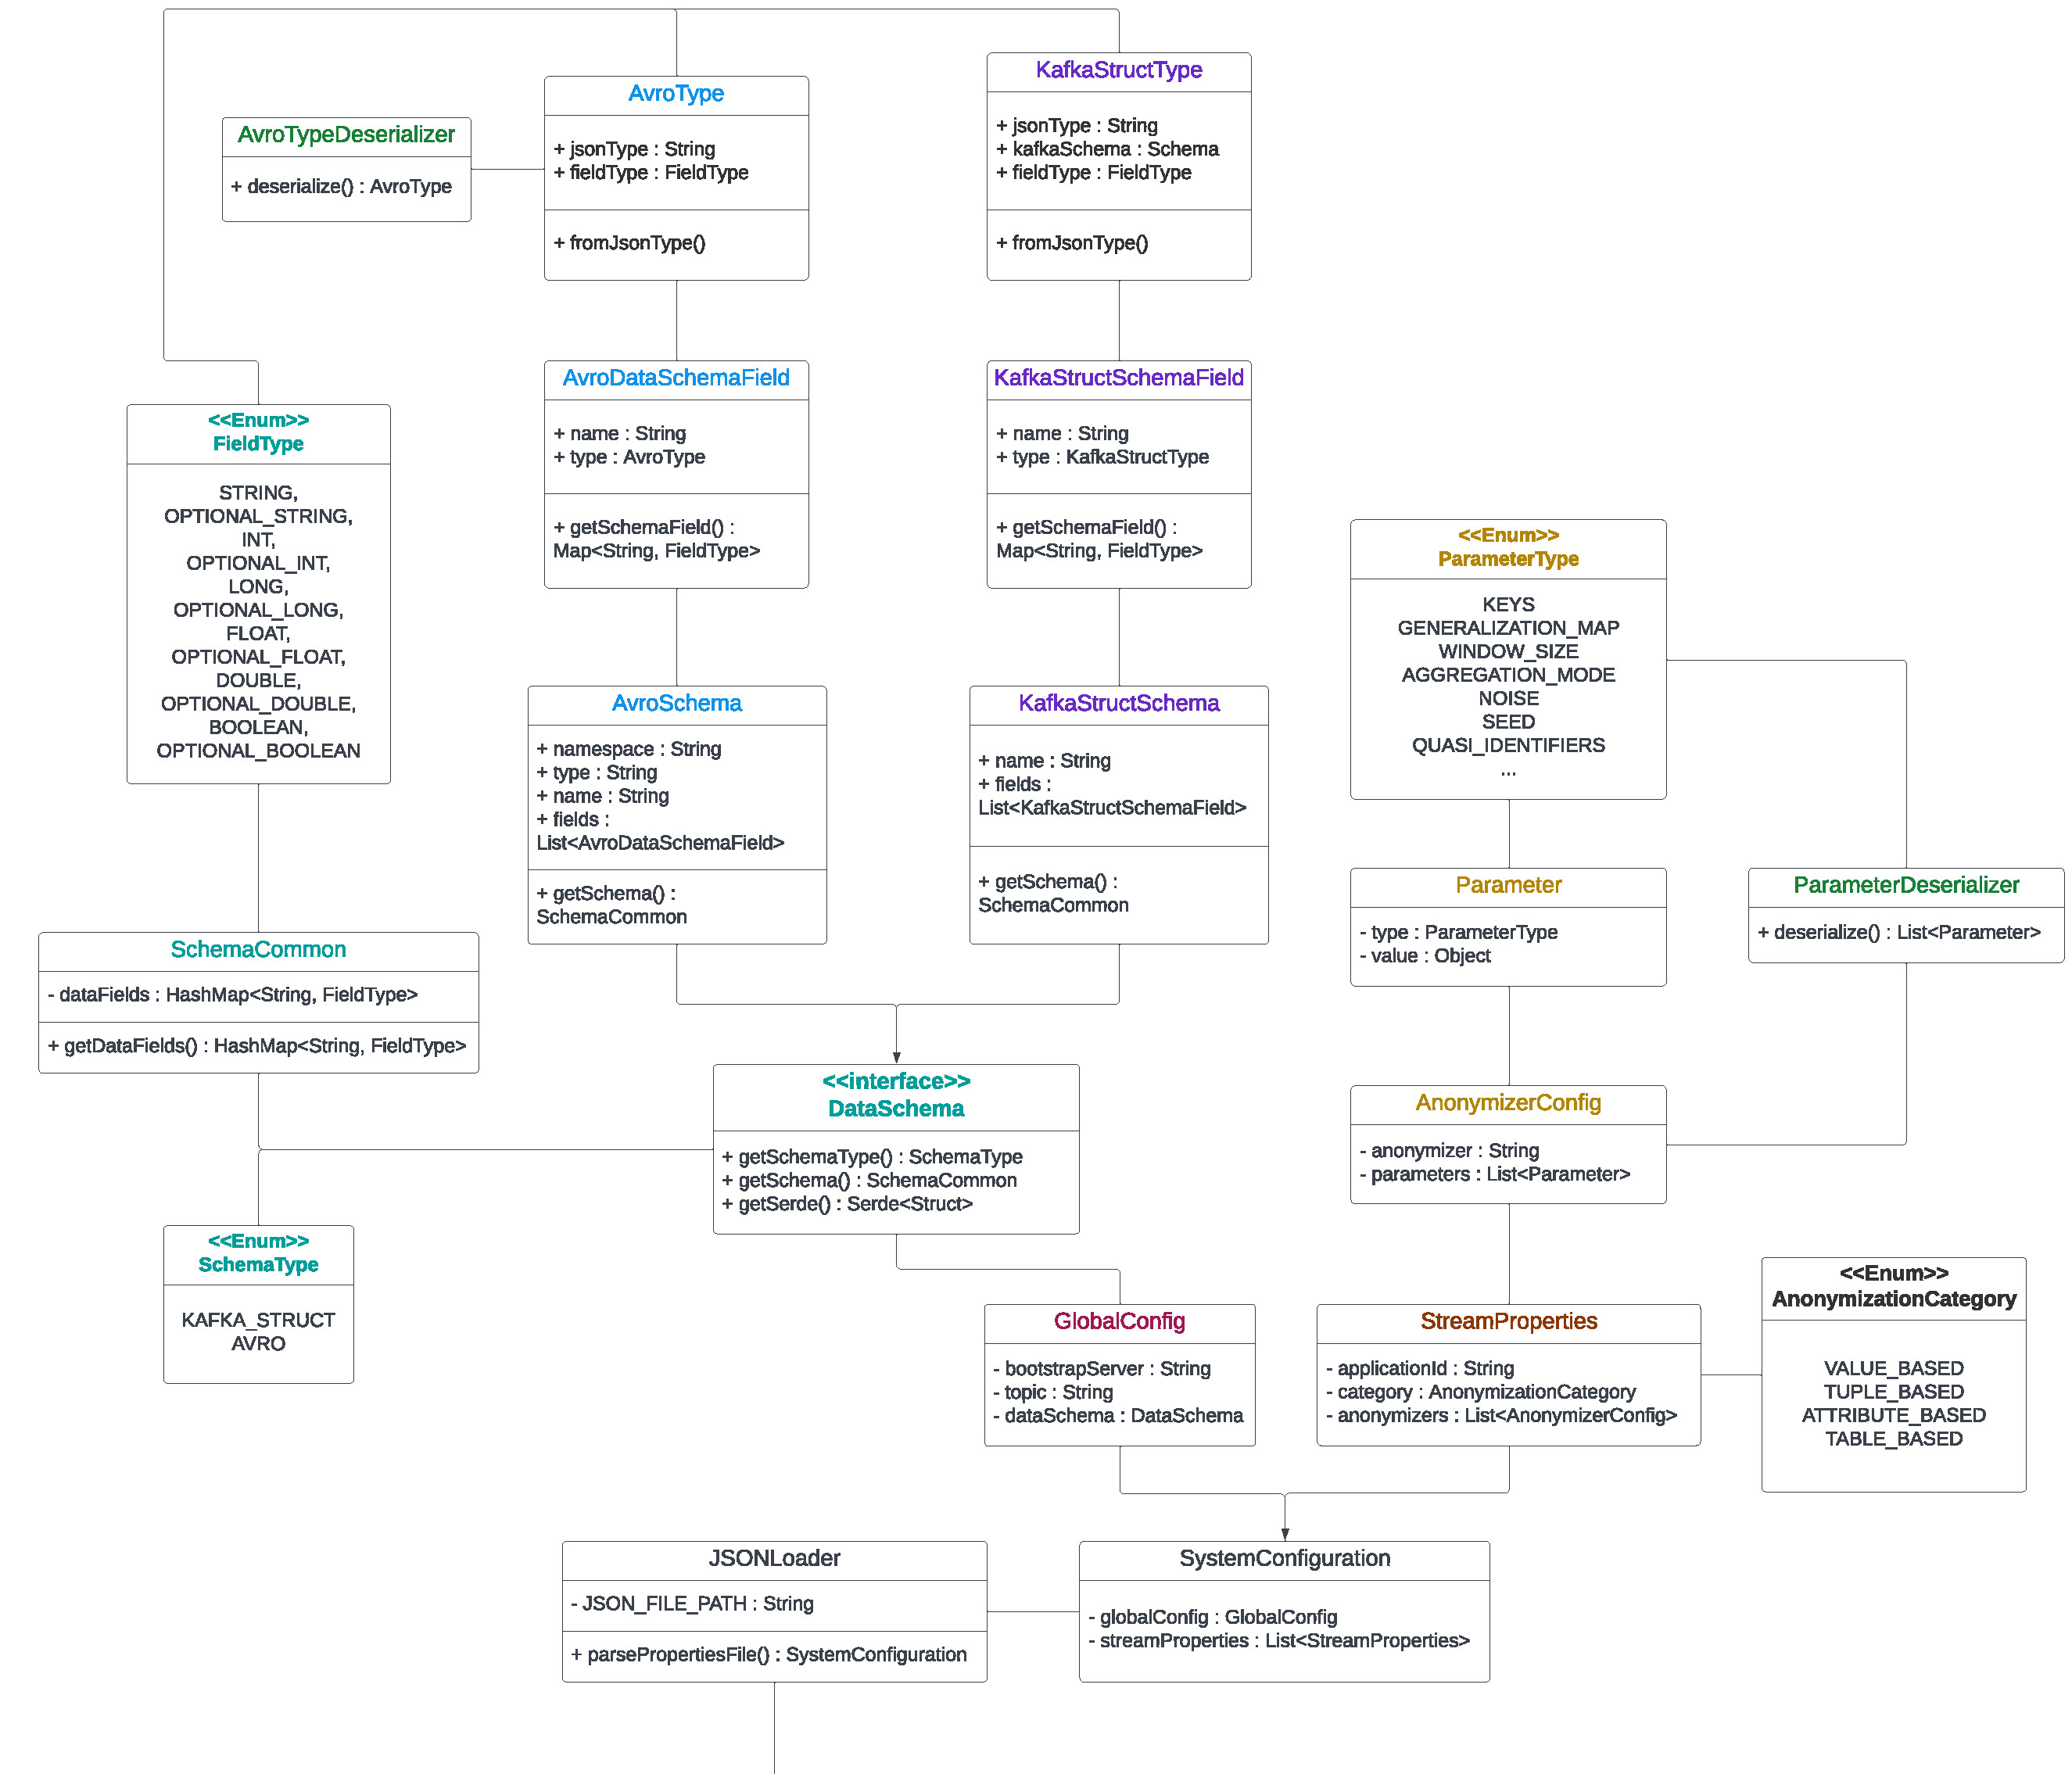
\includegraphics[width=0.85\pdfpagewidth]{img/Requirements_Parser_Class_Diagram.pdf}
   \end{adjustbox}
   \caption{Class Diagram of the JSON Loader responsible for parser the Data Officer's requirements.\label{fig:requirements_parser}}
\end{figure}

Next to the GlobalConfig are the StreamProperties. Each stream includes at least one anonymizer. An anonymizer (highlighted in yellow) is specified with a name and its parameters. All available parameters of all anonymizers are represented as a constant in the ParameterType enum. As one anonymizer can include many parameters of different types a special ParameterDeserializer was implemented. This deserializer processes each parameter in the list individually, converting it into an object as defined by the Parameter class corresponding to that ParameterType. These include simple types like double or int, but can simultaneously be more complex as hierarchies, enums, hashmaps, and lists. Again, \ac{DASH} has been designed to facilitate change. Adding new Parameters is as simple as adding a new value to the ParameterType enum and implementing its deserialization in the ParameterDeserializer.\par
The deserialization relies heavily on the correct format of the requirements and thus provides extensive error messages to the user, the Data Officer, upon failures. Additionally, a recipe with examples as well as documentation - is included in the artifacts found in the thesis repository (\url{https://github.com/TheRealHenri/master_thesis}). Consequently, the JSONLoader accomplishes another crucial task alongside the processing of the configuration, it checks the syntax of the requirements JSON. The deserialization accepts only the expected types for all classes and parameters. A wrong input syntactically will be caught here. The semantics of the requirements, specifically of the parameters, are validated in another component of \ac{DASH} - the Stream Config Builder. 

\subsection{Stream Config Builder}

 
\subsection{Stream Manager}
\subsection{Kafka Streams}

\section{Test Suite}
\subsection{Data Generator}
\subsection{Kafka Connector}
\subsection{Consumers}

\section{Docker}
Putting it all together
Docker compose 
Network 
Volumes
Dependencies
Individual Dockerfiles